\documentclass[11pt,a4paper]{article}
\usepackage[top=3cm, bottom=3cm, left=2.5cm, right=2.2cm]{geometry} %geometry of page
\usepackage[hidelinks]{hyperref} %reference links
\usepackage{fancyhdr} %header and footer control
\usepackage{minted} %source code syntax highlighting
\usepackage{qrcode} %qrcode links
\usepackage{graphicx} %images
\usepackage{parskip}
\linespread{1.3}
\emergencystretch 3em

% Set Header and Footer
\fancyhead{}
\fancyhead[L]{\textbf{Lab 1: Inbuilt LED}}
\fancyhead[R]{max.champneys@sheffield.ac.uk}
\fancyfoot{}
\fancyfoot[L]{\thepage}
\fancyfoot[R]{MAC 233 Arduino Labs, School of MAC, University of Sheffield}

% Create Document
\begin{document}
\pagestyle{fancy}

\section*{Objectives}

The objective of today's lab is to learn how to control an output from the Arduino. We will start with the Arduino's inbuilt LED; in the next lab we will expand this example to control an externally connected LED.

Although the lab today might seem very simple, it will give you the chance to make sure that you can access the Arduino IDE and then write, compile and upload an Arduino sketch to the board. This will help us to diagnose any issues \emph{before} we introduce additional components and complexity.

This worksheet will walk you through the steps of being able to display your name via Morse Code on an LED. Morse code is a method for encoding text as a sequence of dots and dashes. A `Dot' will be represented as turning the LED on for 1 second. A `Dash' will be represented by turning on the LED for 3 seconds. After a `dot' or `dash' is displayed, the LED will need to be off for 1 second before displaying the next `dot' or `dash'.

The basic premise of the sketch is that we have an array (e.g. a vector or list) of signal instructions --- a set of `dots' and `dashes'. The sketch keeps track of where within these set of signal instructions we currently are, so that every time the `loop' function is executed, the LED can turn on for the correct amount of time for the current position within the sequence.

\section{Connecting to your Arduino}
If you do not have the Arduino IDE installed on your computer, please refer to the instructions \href{https://www.arduino.cc/en/software}{\underline{here}}: \url{https://www.arduino.cc/en/software}.

First start by opening the Arduino IDE and creating a blank sketch: `File' \textrightarrow `Examples' \textrightarrow `01.Basics' \textrightarrow `BareMinimum'. Your IDE should now contain a minimum sketch discussed in the first lecture. 

Before writing any code, check that you can get a sketch onto the board. Work through the following steps in order:

\begin{enumerate}
    \item Connect your Arduino to your computer using a USB cable. A light on the board should come on to show it has power.

    \item Tell the IDE which board you are using and which port it is connected to: `Tools' \textrightarrow `Board' \textrightarrow `Select Other Board and Port'. Type \verb|nano every| into the search box, select `Arduino Nano Every' from the \textbf{BOARDS} list on the left, select the matching port from the \textbf{PORTS} list on the right, then click `OK'. You must select \emph{both} --- selecting only a board will let you compile, but not upload.

    \begin{center}
        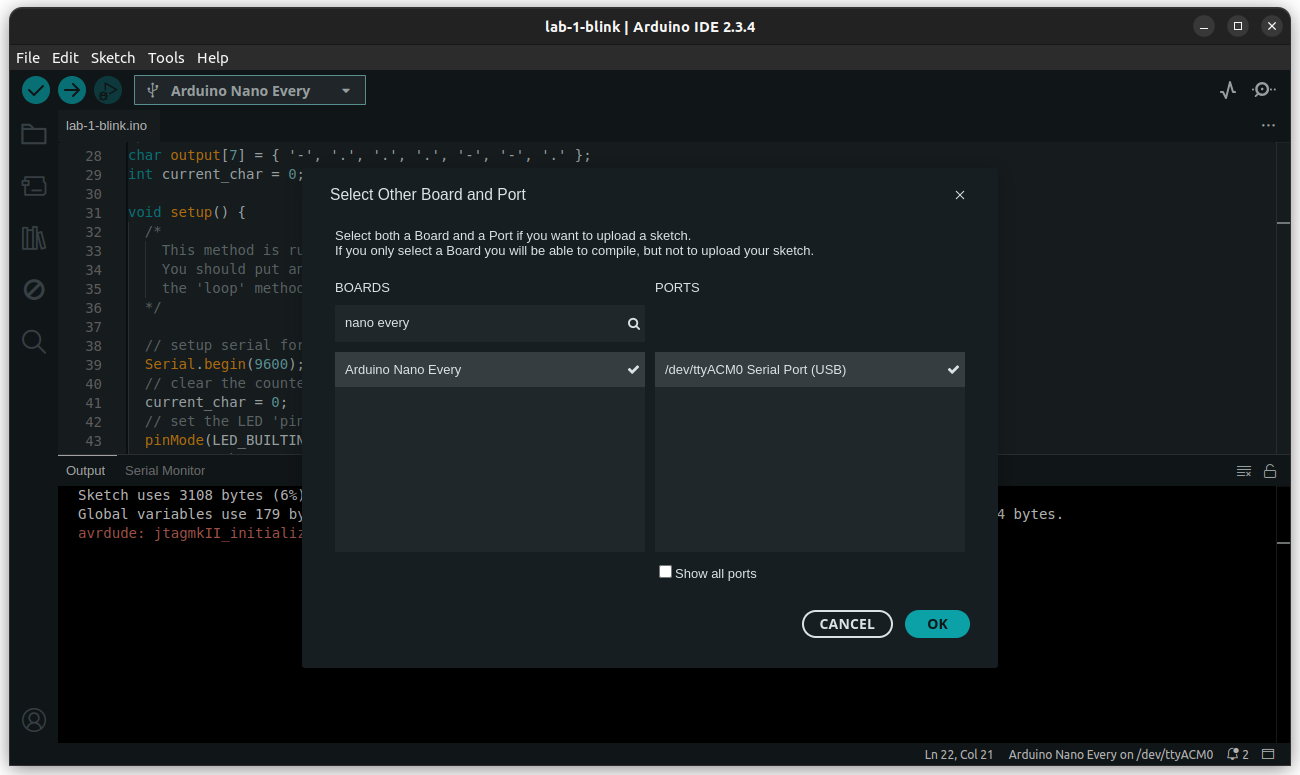
\includegraphics[width=\textwidth]{../images/arduino-board-selection.png}
    \end{center}

    \item Compile the sketch: `Sketch' \textrightarrow `Verify\textbackslash Compile'. This checks your code for errors without sending anything to the board. Fix any errors reported in the black output panel before continuing.

    \item Upload the sketch to the board: `Sketch' \textrightarrow `Upload'. The board manager at the top of the window should read `Arduino Nano Every' in bold; if it does not, repeat step 2.
\end{enumerate}

The `BareMinimum' sketch does nothing, so you will not see any change on the board itself. What matters is that it uploaded without errors: that tells you the IDE, the cable and the board are all working. If you had any problems with the steps above, ask a demonstrator now --- it is much easier to solve before we start adding code and components.

\section{Turning on the LED}
Our first step is to set up the serial connection: this allows us to monitor what the Arduino is doing. Then we can set the internal LED pin to an output mode. The above is done within the `setup' function. Within the main `loop' we set the pin with the LED on to `HIGH'.

% not pulled from the sketch: this is an intermediate state of the build-up,
% before the Morse variables exist, so it appears nowhere in the finished file
\begin{minted}{arduino}
void setup() {
  Serial.begin(9600);
  pinMode(LED_BUILTIN, OUTPUT);
  delay(3000);
  Serial.println("System Ready");
}

void loop() {
  digitalWrite(LED_BUILTIN, HIGH);
}
\end{minted}

Upload this sketch to your Arduino the same way as before (`Sketch' \textrightarrow `Upload'). Then open the serial monitor so you can see the messages the Arduino sends back: `Tools' \textrightarrow `Serial Monitor'. It opens in the bottom section of the IDE, next to the `Output' tab. Set the baud rate drop-down to \textbf{9600} --- this must match the value passed to \verb|Serial.begin| in your sketch, or you will see random characters instead of words.

If everything has worked, your Arduino will power on, wait 3 seconds, display `System Ready' in the serial monitor, and then turn its inbuilt LED on and leave it on.

\section{Add Morse Code variables}
To make our sketch understand Morse Code, we need to add five lines of code within the global scope. \verb|TIME_UNIT| declares that a unit of time is 1000 milliseconds, \verb|DOT_UNITS| says that a `dot' is 1 unit of time, and \verb|DASH_UNITS| that a `dash' is 3 units of time.

\inputminted[
    autogobble, stripnl,
    rangestartstring={\#define TIME_UNIT},
    rangestopstring={int current_char = 0;},
]{arduino}{../lab-1-blink.ino}

\verb|output| is an array (a vector) of 8 `dots' and `dashes' representing the sequence of signals needed for the word `MAX'. The first two (--) represents M, the next two (.-) represents A, and the last four (-..-) represents X. \verb|current_char| stores the current position within the Morse code sequence, initially zero.

\section{Process the Morse Code message}
We now need to modify the main `loop' function to correctly process the Morse code message. This is broken down into three stages: calculate the duration to turn the LED on for (see Section \ref{sec:duration}), turn the LED on for the desired duration (see Section \ref{sec:led}), and lastly calculate the next signal to display (see Section \ref{sec:next}).

Before continuing to the next sections, we first need to remove the existing `digitalWrite' line from `loop' function so that it is empty.

\subsection{Calculate the duration}
\label{sec:duration}
At the beginning of the `loop' function, we need to enter the code to calculate the duration to turn the LED on for. This is based upon the \verb|current_char| variable which tracks the position within the signal sequence (the \verb|output| variable).

If the current position within the sequence equals a `.' then we need to set the LED (\verb|led_on_time|) to be on for 1 time unit; however, if the current position within the sequence equals a `-', then we need to set the LED to be on for 3 time units.

\inputminted[
    autogobble, stripnl,
    rangestartafterstring={// calculate amount of time LED is to be on for},
    rangestopbeforestring={// turn the LED on and off},
]{arduino}{../lab-1-blink.ino}

\subsection{Turn on the LED}
\label{sec:led}
The next logic within the `loop' function needs to be turning on the LED, waiting for the desired duration calculated in the previous step, then turning the LED off again.

\inputminted[
    autogobble, stripnl,
    rangestartafterstring={// turn the LED on and off},
    rangestopbeforestring={// determine the next sequence to display},
]{arduino}{../lab-1-blink.ino}

The `digitalWrite' function is a key action you will often use during these labs. It allows us to write a `HIGH' or `LOW' value to something connected to the Arduino; in our case of an LED, this is an ON and OFF signal. The `delay' is another key function that enables you to pause the sketch on the Arduino for $n$ milliseconds. 

\subsection{Calculate the next signal}
\label{sec:next}
Once you have displayed the current signal to the LED, the final piece of logic within the `loop' function is to calculate where within the sequence the next iteration of the `loop' should go.

The logic for this is that if your current signal being displayed is the last signal in the sequence, then you need to start back at zero, else go to the next signal in the sequence.

\inputminted[
    autogobble, stripnl,
    rangestartafterstring={// determine the next sequence to display},
    rangestopstring={delay(TIME_UNIT);},
]{arduino}{../lab-1-blink.ino}

The last line is the gap between signals. It leaves the LED off for one time unit after each `dot' or `dash', so that two signals in a row do not run into one another --- the 1 second pause described at the start of this worksheet.

\section{Try it out on your Arduino}
Now that you have the above sections complete in your sketch, compile and upload the sketch to your team's Arduino.

Once you have successfully run this sketch on your Arduino, change the sequence displayed to the name of one member from your team. You can find a Morse code chart on the Wikipedia page: \url{https://en.wikipedia.org/wiki/Morse_code}.

Note: the code included within this lab assumes that the Morse code message will only ever be a sequence of 8 signals. Can you change your code to work no matter how long the sequence of signals is?

\section*{Help}
If you are having issue compiling the project or don't understand where each section goes, you can see a complete version of the sketch with additional source code comments at \url{https://github.com/MDCHAMP/MAC233/blob/main/labs/lab-1-blink/lab-1-blink.ino}.

\vspace{2em}

\begin{center}
    \qrcode[hyperlink, height=6cm]{https://github.com/MDCHAMP/MAC233/blob/main/labs/lab-1-blink/lab-1-blink.ino}
\end{center}


\end{document}